\chapter{Revue de litterature}

	Ce chapitre permet de mettre en revue la thématique du big data et de l’intelligence artificielle en utilisant les ouvrages, articles édités auparavant. Cette revue de littérature met l’accent sur leur impact  dans l’éducation en milieu scolaire.
	
\section{Intelligence artificielle dans l’éducation }

De nos jours, nous avons une nouvelle éducation de la data par la data car elle a toujours été présente, elle est juste plus explicite aujourd’hui : les données étant produites et générées par certaines plateforme, on le sait et c’est pourquoi on ouvre de nouveaux espaces pour réfléchir à quelle quantité de données doit être utilisée pour la personnalisation, pour ce modèle d’apprentissage axé sur l’inconnu. 

\subsection{L’intelligence artificielle}

Bien que pensé il y a longtemps, l’histoire de l’IA n’est pas récente. Tenter de programmer une machine pour qu’elle interprète un langage et les concepts abstraits de façon à ce qu’elle résolve des problèmes jusqu’alors réservés aux humains est un projet bien ambitieux. L’IA pourrait se définir de nombreuses façons  qui tiennent tant des objectifs du champ que des conditions qui sont posées pour la départager d’autres applications informatiques. Depuis 2010, les succès de l’IA sont dus aux approches du machine learning et du deep learning, succès rendu possible grâce à l’augmentation des puissances de calculs et de stockage, ainsi qu’à la disposition des mégadonnées (big data); termes fréquemment  retrouvés dans des articles d’actualité. Ce vocabulaire généralement utilisé dans le monde de la recherche, se vulgarise au grand public de jours en jours; et pour cause, l’on observe leur émergence au sein des entreprises par des services conçus à partir des solutions d’IA. Celles-ci suscitent un intérêt pédagogique et scientifique croissant depuis une trentaine d’années qui s’est accélérée récemment à la suite des performances de ses techniques. Alors, nous devons avoir un minimum de connaissance dans celle-ci pour autant qu’elle s’insère dans nos produits de consommation tels que les smartphones, tablettes, … (tel que Alexa de Google ou encore Siri de Apple). Ceci laisse penser que la vulgarisation entraînera un changement non pas seulement dans nos habitudes de travail, mais également dans le quotidien et donc une dépendance d’où selon le point de vue de certains chercheurs (Stephen Hawking; « Le développement d'une intelligence artificielle intégrale pourrait signifier la fin de la race humaine. »), cette technologie pourrait déterminer l’avenir de la race humaine dans sa formule la plus élevée. Dans leur revue systématique de littérature, Zawacki-Richter et al identifient quatre applications principales de l’IA en enseignement supérieur : 

\begin{itemize}
	\item le profilage et la prédiction (admission à un programme d’étude, décrochage scolaire) ,
	\item Les systèmes de tutorat intelligent (enseignement de contenus pédagogique, rétroaction), 
	\item La mesure et l’évaluation (notation automatique, engagement scolaire) et 
	\item les systèmes adaptatifs et personnalisés (recommandation et sélection de contenus personnalisés)
\end{itemize}

En revanche, les enjeux éthiques et critiques que soulève l’IA sont peu étudiés en enseignement supérieur et en éducation plus largement. Souhaitant contribuer à cette émergence, nous proposons d’abord quelques enjeux éthiques et critiques de l’IA, sans toutefois prétendre à l’exhaustivité, ainsi que de formuler quelques pistes d’action permettant de mieux les prendre en compte, tant du point de vue de la conception que de l’usage. 

\subsection{Les enjeux éthiques et critiques de l’intelligence artificielle liés à l’éducation}

\subsubsection{Enjeux liés aux données massives}

	Le lien entre le big data et l’intelligence artificielle est important. Les écosystèmes qui recueillent un grand nombre de données permettent aux systèmes qui ont recours à l’IA de les exploiter. Les enjeux éthiques et critiques liés au big data que nécessitent l’IA peuvent induire des biais éventuels et posent la question de la vie privée sur les acteurs d’école scolaire. C’est le cas par exemple de la suite éducative Google, qui collecte des données sans consentement libre des élèves et du personnel scolaire (en contradiction avec leur politique et celle des Etats) et les exploite de manière opaque. Les données du personnel et des élèves sont donc utilisées à leur insu, causant ainsi un manquement au respect de leur vie privée. 
	
	\subsubsection{Enjeux liés aux algorithmes}
	Les algorithmes sont au cœur de l’IA. Il s’agit d’une suite d'instructions visant à définir le comportement d’un système pour permettre d’obtenir un résultat à partir de données fournies en entrée. Parfois confronté à des algorithmes si complexes qu’on ne peut résoudre de façon optimale à l'instant t, il est nécessaire d’utiliser des algorithmes heuristiques qui produiront des solutions pas nécessairement optimales mais qui feront l’affaire à cet instant. Par ailleurs, l’IA principalement produite par des entreprises privées plutôt que des instances scolaires génère des enjeux éthiques  et critiques relatifs aux expertises et représentations éducatives mobilisées par les équipes de conception. En dehors de l’éducation, plusieurs études ont déjà souligné le manque de diversité au sein des équipes de conception, ce qui se traduit par des biais de représentativité allant de la sous-représentation de certains groupes sociaux à leur discrimination, stigmatisation ou exclusion. Ceci s’observe en 2015 avec l’algorithme de Google photos qui associe une photo de deux personnes noires américaines au tag “gorilles”. faute d’avoir été suffisamment entraîné à identifier des visages à la peau foncée. 

\subsubsection{Enjeux relatifs à l’autonomie et au jugement professionnels des enseignant(e)s et à l'agentivité des élèves en fonction de la distribution des tâches entre eux et l’IA}

Les systèmes de gestion des comportements permettent aux enseignant(e)s de documenter les comportements nuisibles des élèves qui sont ensuite compilés et signalés automatiquement à l’administration scolaire en vue d’appliquer des conséquences proportionnelles. Faute de temps en salle de classe, certain(e)s enseignant(e)s documentent les comportements après les cours, parfois sans en avoir informé les élèves concernés. Les élèves peuvent donc être mis.es en retrait pour une suite de comportements nuisibles dont elles ou ils n’ont pas souvenir, ce qui met à mal les principes mêmes de cohérence et de justice, en éducation.

\subsubsection{Vers une écologie de l’attention }
A l’ère du 21e siècle, la technologie, dont l’IA devient indispensable. Mais les utilisateurs commencent à se rendre compte des différentes dérives de ces outils numériques. D’où la question: Si elle était mieux connue, la manipulation de l’attention à des fins commerciales serait-elle socialement acceptée? Il est question ici d’amener l’utilisateur à être conscient de l’impact de son utilisation du numérique sur son bien être physique et psychologique. 

\subsection{Prévenir les enjeux de l’intelligence artificielle}
	De ces types d’enjeux éthiques et critiques, il est possible d’esquisser quelques pistes de réflexion et d’action. En premier lieu, ces enjeux gagnent à être pris en compte dès la phase de conception, afin de prévenir autant que possible des retombées négatives éventuelles lors de l’usage. On peut alors se poser la question suivante : dans quelle mesure les équipes de conception intègrent-elles des expertises et des représentations éducatives lorsqu’elles développent des technologies impliquant l’IA ? Un premier pas pour s’en assurer consiste, pour les équipes de conception, à opter pour des modèles centrés usager » dans le but de maximiser la prise en compte des expertises et des représentations éducatives et de préserver la finalité éducative des finalités économiques et techniques. Un pas supplémentaire consiste à adopter et respecter des principes éthiques de conception, comme le fait d’informer systématiquement et explicitement les usagers lorsqu’elles ou ils sont en interaction avec un système d’intelligence artificielle. Sur le plan de l’usage, sensibiliser les élèves et le personnel scolaire aux enjeux de l’IA en éducation implique d’intégrer une dimension éthique et critique explicite à la formation aux technologies. Pour être complète, cette dimension gagnerait à ne pas se limiter aux « bons usages » de l’IA, mais à s’articuler autour de la compréhension des interactions entre la conception et l’usage de l’IA d’une part, et entre les usages et leurs implications éducatives et sociales d’autre part. Par exemple, le modèle techno éthique de Krutka et al. (2019) ouvre une voie intéressante en formation initiale et continue des enseignants : pour déterminer si une technologie donnée est éthique, il propose une analyse des dimensions éthique, légale, démocratique, économique, technologique et pédagogique, guidée par des questions, ainsi que des éléments à considérer et des applications pratiques à intégrer à la formation des enseignants.

\subsection{Possibilités et défis pour l’éducation}
L’IA, ne possédant pas (encore) les qualités humaines propre à la profession (jugement critique, empathie, bienveillance, ...), l’enseignement pourrait faire parti des emplois les moins menacés de disparition bien qu’elle ait marqué un pas avec l’apprentissage adaptative mais le personnel enseignant sera de plus en plus appelé à jouer un rôle de conseiller, de guide et d’accompagnateur. 

\subsubsection{Des exemples d'application de l'IA en éducation}

Elle s’utilise de plusieurs façons dont:  
Les systèmes tutoriels intelligents qui s’adaptent en temps réel aux capacités et aux besoins de la personne en formation
Les tests corrigés automatiquement qui fournissent des informations utiles sur les compétences et aptitudes qu’elles ont développées.
Les environnements d’apprentissage collaboratif 
Les enjeux visant l’apprentissage, 
D’où elle marque un pas important avec l’apprentissage adaptatif selon le profil de l’apprenant, ce qui favorise la différenciation pédagogique.  \\ 
Le schéma de VTE est plus explicite sur le processus d'adaptation de l’IAED  
	\begin{figure}[hbtp]
	\centering
	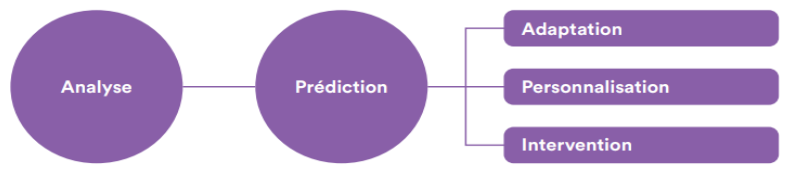
\includegraphics[scale=0.7]{../img/VTE.png}
	\caption{Schéma d'un VTE}
	\end{figure} 
	\\
	\\
	\\
	\\
	\\
	
	Bien que l’IA propose des outils pour améliorer l’apprentissage, il n’en demeure pas moins qu’il s’agit d’une technologie qui a des répercussions sur notre vie quotidienne et à l’égard de laquelle nous devons demeurer critiques.\\

\subsubsection{Des compétences à développer}
Pour répondre à des défis éducatifs, il est nécessaire d’éduquer les individus sur l’IA ainsi qu’à l’IA l’intelligence humaine (Éduquer à l’IA qu’avec l’IA) vu qu’elle augmentera la nécessité de développer de nouvelles compétences ce qui pourrait provoquer une pénurie d’enseignants mais aidera tous les élèves à réaliser leur potentiel.

\noindent

La principale contribution de l’IA au logiciel d’éducation est la modélisation de l’expertise. L’expertise est la capacité pour le système expert de résoudre les systèmes complexes que les apprenants doivent résoudre. \\
On peut modéliser l’expertise de 04 manière :
	\begin{itemize}
		\item L’interaction : le processus de résolution du problème est découpé par étape intermédiaire 
		\item L’explication : la méthode utilisée pour résoudre le problème est décrite ici en langage naturel
		\item Le Diagnostic : cette méthode analyse les réponses de l’apprenant pour établir des propositions à propos de ses connaissances : ce qu’il sait et ce qu’il ne sait pas.
		\item Le curriculum : Cette méthode décide quel concept ou compétence à enseigner à l’apprenant sur la base de son comportement 
	\end{itemize}
	
	En conclusion, modéliser l’expertise permet au système de fixer le problème avec l’apprenant, de négocier les étapes intermédiaires, d’expliquer les décisions et de raisonner sur la connaissance de l’apprenant; on dit que le système résonne avec l’apprenant. L’IA, vu comme un outil pour mieux apprendre, est le premier usage  auquel on pense. Utiliser des algorithmes d’intelligence artificielle pour proposer des outils afin de mieux apprendre, optimiser le rendement de l’apprenant. Le point clé est l’apprentissage adaptatif.
 


\section{Apprentissage adaptatif}

\subsection{Qu’est-ce que c’est?}


L’apprentissage adaptatif est une tendance émergente en enseignement supérieur. Il repose sur des cours, des exercices et des évaluations  qui s’ajustent en temps réel aux besoins d’un apprenant. L’adaptation est réalisée en temps réel grâce à des algorithmes qui font des inférences à partir des actions de l’apprenant en session d’apprentissage. Un exemple d’inférence est le diagnostic de leurs erreurs. Plus la machine simule le comportement d’un tuteur humain, plus elle est dite \quotes{intelligente}. On parle alors de tuteur intelligent et d’apprentissage adaptatif intelligent.\\ Le caractère \quotes{intelligent} d’un environnement d’apprentissage réside dans le fait qu’il puisse s’adapter à l’apprenant. Par adaptabilité, on entend la capacité de l’environnement d’apprentissage à modifier son comportement à partir d’inférences effectuées en fonction du contenu actualisé d’un modèle de l’apprenant, que ce soit sur son état cognitif, métacognitif ou affectif. 

\noindent

 L’adaptabilité d’un environnement d’apprentissage intelligent (EAI) est mise en œuvre grâce aux données éducatives qui y sont collectées. Elles correspondent généralement à des informations : \\
	-  Sur le profil de l’apprenant, la stratégie pédagogique et le domaine d’apprentissage ;\\
	-  Provenant de la saisie des interactions de l’apprenant avec l’interface de l’ \acrshort{eai}.\\
   Ces données sont généralement utilisées pour :\\
	-  Planifier dynamiquement les objectifs et les activités d’apprentissage dans l’ \acrshort{eai} ;\\
	-  Configurer son interface, la présentation et la séquence des activités ; \\
	-  Guider l'apprenant lors d'une activité ; \\
	-  Établir un diagnostic cognitif de l’apprenant.

\subsection{Architecture et composition d’un système d’apprentissage adaptatif}

Les systèmes d’apprentissage adaptatif sont généralement divisés en différentes composantes ou \quotes{modèle}. Différents groupements de modèles ont été présentés, et la plupart des systèmes incluent une partie ou l’ensemble des modèles suivants : \\
	- Le modèle expert ou modèle de domaine : le modèle contient l’information qui est à enseigner \\
	- Le modèle apprenant : le modèle relève les traces de l’apprenant et enregistre sa progression (personnaliser l’apprentissage en tenant compte des particularités de l’apprenant)\\
	- Le modèle d’instruction ou modèle pédagogique : le modèle décide effectivement ce qu’il y a à apprendre \\
	- Environnement : c’est l’interface avec laquelle l’utilisateur interagit avec le système. Il constitue la couche de communication (les interactions) entre l’apprenant et le système. \\
	Ils sont résumé sur l'architecture des ITS suivante:
	
	\begin{figure}[!ht]
		\centering
		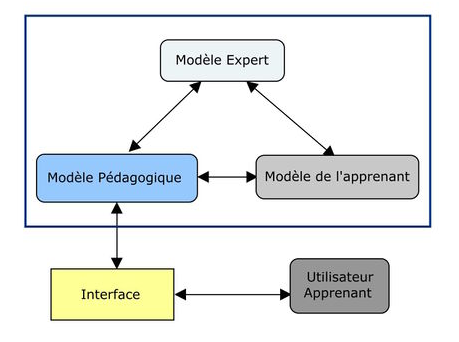
\includegraphics[scale=1]{its.png} 
		\caption{Architecture ITS}
		\label{ferme}
	\end{figure}


\section{Système de recommandation}

\subsection{Définition}

	Un système de recommandation est un moteur qui produit des recommandations individualisées ou qui a pour effet de guider l’utilisateur de manière personnalisée vers des contenus  intéressants ou utiles parmi de nombreuses options possibles. Ces outils font déjà partie intégrante de notre vie quotidienne. Ceux-ci se glissent plus ou moins discrètement dans nos vies numériques et rythment notre quotidien lors de nos navigations sur le web. Nous n’en sommes pas tous conscients, pourtant, la recommandation de contenu est omniprésente dans tous les grands secteurs d’activités numériques, par exemple : le e-commerce, la presse en ligne, les services de streaming vidéo et musical et bien entendu les réseaux sociaux y ont aussi massivement recours. \\

  	\textbf{→  Pourquoi utiliser des algorithmes de recommandation?} \\
	Si tous les grands acteurs de ces secteurs ont vite saisi les opportunités offertes par l’immensité de données mise à disposition par les internautes, c’est que les algorithmes de recommandation sont utiles à bien des fins : 
   \begin{itemize}
	\item Amélioration de l’expérience utilisateur 
	\item Augmentation continue des performances clés (durée de visionnement, temps de lecture, panier moyen, raccourcissement des délais de recherche de contenus/produits, etc.)
	\item Gestion d’un volume croissant de données impossible à traiter manuellement 
	\item Analyse pointue des données pour des recommandations personnalisées pertinentes
	\item Automatisation du filtrage des données
   \end{itemize}

\subsection{Les catégories de système de recommandation  }

	\subsubsection{Le filtrage collaboratif }
Il repose sur l’adage qui stipule: \quotes{Si deux personnes ont aimé des contenus identiques par le passé, elles ont une probabilité élevée d’aimer les mêmes choses dans le futur.} C’est actuellement l’un des moyens les plus performants quand il s’agit de faire de la recommandation à des lecteurs déjà connus. 

	\begin{figure}[!ht]
		\centering
		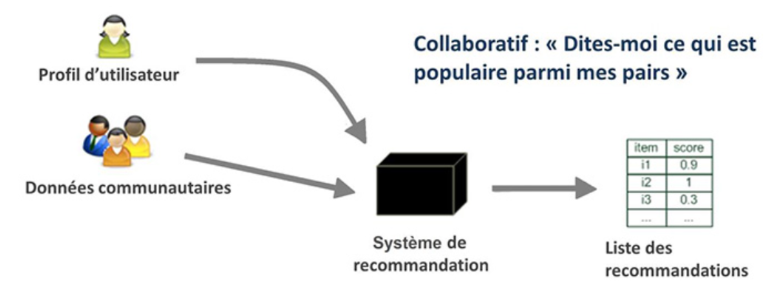
\includegraphics[scale=1]{src.png} 
		\caption{Système de recommandation collaboratif}
		\label{ferme}
	\end{figure}

Les recommandations personnalisées issues du filtrage peuvent être déterminées de plusieurs manière, notamment: 
 \begin{itemize}
 	\item[$\star$] Sur le profil des lecteurs (User-based)
 \end{itemize}
 Il repose sur le principe : si des lecteurs ont des comportements et goûts de lecture similaires par le passé, alors, ils devraient également en avoir dans le futur. L’avantage du filtrage collaboratif est qu’il est agnostique au contenu. Il se base uniquement sur le profil de navigation des lecteurs pour faire des recommandations personnalisées.

 \begin{itemize}
 %	\item[$\star$] Sur les profiles de contenus (Item-based)
 \end{itemize}
 Cet algorithme fonctionne un peu comme le user-based, mais utilise les similarités entre les profils d’articles pour proposer les recommandations aux lecteurs. Pour identifier les similarités entre articles, l’item-based utilise un profil d’article qui est constitué de la liste des utilisateurs ayant lu/aimé cet article. Les articles identifiés comme similaires à un article donné parce que les mêmes gens les ont aimés sont alors recommandés aux gens qui ont lu cet article. 
 \begin{itemize}
 	\item[$\star$] Sur la factorisation de matrice
 \end{itemize}
 On peut voir la liste des profils utilisateurs comme une matrice. Typiquement, la ligne u contient la liste des articles aimés par u, la colonne a contient la liste des utilisateurs qui ont aimé a. L’objectif d’un algorithme de recommandation est de remplir les cases vides de cette matrice. 
 
\noindent 

Un problème de factorisation matricielle est un problème d’optimisation où l’on suppose que le modèle M est le produit de matrices de facteurs latents, comme par exemple Mi j = \{ U? i ,V ? j \}, où U? i est le vecteur (de taille d) des variables latentes explicatives de l’utilisateur i et V ? j est le vecteur des variables latentes explicatives de l’article j.  Généralement, on considère que le nombre de variables latentes d est très inférieure à la taille des données. Le but de la factorisation matricielle est d’estimer ces matrices U? et V ? afin d’obtenir une reconstruction qui jouera le rôle de fonction score Mˆ i j = \{ Ui ,Vj \}. Le principal intérêt de la factorisation (particulièrement dans la recommandation) est de fournir une représentation de faible rang d’un modèle de grande dimension.
	
	\subsubsection{Le filtrage de type “Content based”}
	Ici, l’algorithme analyse un ensemble de contenu sans prendre en compte les utilisateurs (en tout cas, pas dans un premier temps) et détecte les similarités entre les contenus à des fins de recommandation en inspectant son contenu. L’analyse de contenu consiste par exemple à identifier le sujet d’un contenu en répertoriant tous les mots d’un article de presse (excepté les stop words) puis en comparant tous les mots de l’article analysés aux autres articles. Plus un article aura un nombre de mots similaires, plus ces articles seront considérés comme \quotes{proches} permettant ainsi de détecter les sujets identiques ou similaires et d’en déduire des recommandations pour le lecteur.
	\begin{figure}[!ht]
		\centering
		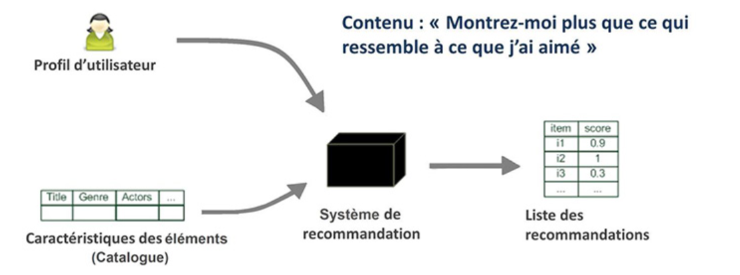
\includegraphics[scale=1]{srbc.png} 
		\caption{Système de recommandation collaboratif}
		\label{ferme}
	\end{figure}
	
	\subsubsection{Les approche hybrides }
	Un système de recommandation hybride utilise des composants de différents types d’approches de recommandation ou s’appuie sur leur logique. Par exemple, un tel système peut utiliser à la fois des connaissances extérieures et les caractéristiques des éléments, combinant ainsi des approches collaboratives et basées sur le contenu. 
	
\noindent

	Le terme \quotes{hybride} est un artefact de l’évolution historique des systèmes de recommandation où certaines sources de connaissances ont été exploitées en premier lieu, conduisant à des techniques bien établies qui ont ensuite été combinées. L’objectif est alors de s’appuyer sur des sources de connaissances multiples, en choisissant les plus appropriées à une tâche donnée afin de les utiliser le plus efficacement possible. \\
		
	\begin{figure}[!ht]
		\centering
		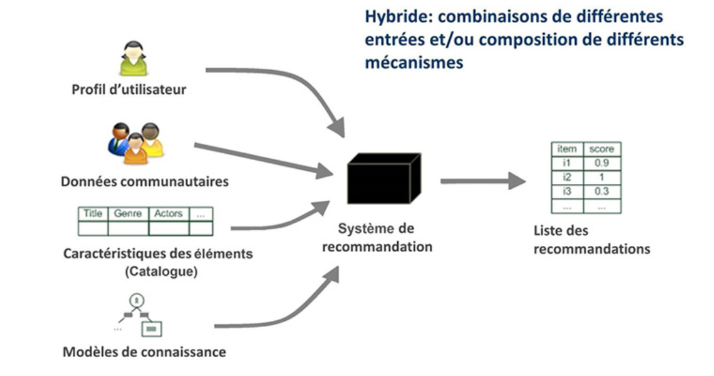
\includegraphics[scale=1]{srh.PNG}  
		\caption{Système de recommandation hybride}
		\label{Système de recommandation hybride}
	\end{figure}


\subsection{L’éthique et les systèmes de recommandation}
	Il nous semble important d’évoquer les problèmes éthiques soulevés dans le monde de la recommandation.\\ De nombreuses polémiques ont eu lieu quant à la façon dont étaient recueillies, stockées ou utilisées certaines données sur les utilisateurs ; en effet, la personnalisation des recommandations est d’autant plus précise qu’elle utilise des données pertinentes sur l’utilisateur, ses goûts et ses comportements. Or l’acquisition et le stockage de données personnelles peut s’avérer intrusive et constituer une violation de la vie privée, notamment lorsque les informations sont collectées de manière implicite à l’insu de l’utilisateur (sans parler des risques de divulgation inopportune de ce type d’information). De plus, l'absence de transparence des entreprises quant à l’utilisation de ces données ou à la façon dont sont réalisées les recommandations n’est en rien rassurante pour les utilisateurs. On peut notamment citer Google qui est poursuivi en juin 2013 par la CNIL 8 pour la façon jugée illégale de collecte d’informations des utilisateurs et pour l’absence de transparence de l’utilisation qui est faite de ces informations. Netflix a également fait l’objet d’une plainte en décembre 2009 pour avoir libéré les données du challenge bien qu’aucune information personnelle n’y figurait. 
	
\noindent
	
	De plus, la connaissance de l’utilisateur par le système de recommandation pourrait aller jusqu’à la personnalisation d’une véritable stratégie d’influence [11]. Un système de recommandation se doit, en plus de respecter la législation, d’être transparent sur sa façon d’effectuer les recommandations pour éviter son rejet par les utilisateurs. Ainsi il devient fréquent de se voir justifier la suggestion d’un article par des phrases du type « les utilisateurs qui ont acheté ce produit, ont également acheté tel produit » rassurantes pour l’utilisateur, qui voit ainsi comment sont utilisées les informations dont disposent les entreprises. Il reste cependant beaucoup à faire, principalement sur le manque de transparence au niveau de la collecte des données et sur leur utilisation. 
 
\subsection{Les systèmes de recommandation en éducation}
 
	Un survol de la littérature met rapidement en évidence la pluralité et la diversité des système de recommandation en éducation. Ces modèles se regroupent en trois typologies: 
	
  	\textbf{\textit{→ Les systèmes de recommandation pour guider les apprenants }} \\
	Il existe plusieurs systèmes de recommandation dans l’apprentissage, l’intérêt de mettre en place un système de recommandation  sur une plateforme d’apprentissage  (type LMS [12], LXP, etc.) est de guider l’apprenant dans son parcours pédagogique en évitant de le surcharger d’informations inutiles. Ces recommandations sont adaptées à ses besoins et ses caractéristiques comme son niveau de maîtrise, ses connaissances antérieures, ses capacités cognitives, ses compétences, et cela afin de l’aider à progresser. \\
	
	
	  \textbf{\textit{→ Le traitement automatique du langage naturel pour la gestion des contenus pédagogiques}} 

\noindent

	Le traitement automatique du langage naturel (TALN), traduit littéralement Natural language processing en anglais (NLP) est un des domaines qui évolue le plus rapidement. Cette discipline de l’IA permet de traiter des données liées au langage que nous utilisons habituellement au format textuel avec les outils de traduction automatique, ou bien vocale avec les assistants vocaux (Siri, Alexa ou Google Home, pour n’en citer que quelques-uns). Le secteur de l’apprentissage foisonne de ressources pour l’utilisation du TALN avec des contenus de formation variés (cours, questions, livres, vidéos, etc.). Ses cas d’applications sont nombreux et peuvent bénéficier aux différents acteurs de la formation, du concepteur de contenu jusqu’au formateur en passant par l’apprenant. On compte parmi les applications possibles : \\
	- La classification de contenus similaires sous une même thématique à l’aide d’algorithmes d’apprentissage supervisés \\
	- La génération automatique de questions à partir de plusieurs corpus de textes
	- La création de synthèses et de résumés de contenu
	- L’aide à la correction en mettant par exemple en évidence les passages liés à certains mots-clé. \\
	Exemple: ProfessorBob.ai, assistant de ... développé depuis 2018
	
	\textbf{\textit{→ Le clustering pour mieux comprendre les apprenants et leurs besoins }} \\
	Le clustering consiste à séparer des éléments en groupes homogènes selon certaines caractéristiques communes. Ce type d’algorithme est utilisé dans des contextes pédagogiques, il permet par exemple de regrouper des apprenants pour faire apparaître des groupes de personnes présentant des difficultés ou au contraire d’autres qui seraient plus avancés sur une compétence à acquérir. Ce type d’information s’avèrera utile pour le formateur qui, en fonction des résultats, pourra offrir un accompagnement plus personnalisé à chaque apprenant. Le clustering peut également être utilisé pour prédire de futurs comportements comme le décrochage, ce qui permet au formateur d’avoir “un pas d’avance” dans son suivi particulier des apprenants.\\
	Exemple: ProfessorBob.ai, un assistant

	%Les systèmes de recommandation aident l'utilisateur individuel à prendre des décisions parmi les vastes choix disponibles en recommandant le ou les choix appropriés en fonction du comportement ou des opinions d'un groupe présentant des caractéristiques ou comportements similaires. 
	%Récemment, certains systèmes de recommandation ont été appliqués dans le domaine de l'apprentissage en ligne. 
%	\subsection{Présentation}
%	Parmi les solutions existantes, nous avons trouvé Adaptiv’Math et rofessorBob.ai, Maths 6e qui sont de très bons outils de :
%	
%\noindent
%
%	\textbf{Adaptativ’Math :} développée dans le cadre du P2iA (Partenariat d’innovation sur l’intelligence artificielle), est un assistant pédagogique pour l’enseignement et l’apprentissage des élèves de cycle 2 (CP au CE2) et une ressource d’apprentissage adaptatif au service de la différenciation pédagogique dont l’ objectif est de co-construire une intelligence artificielle réellement au service des enseignants et de leurs élèves.
%	
%\noindent
%
%	\textbf{ProfessorBob.ai :}  programme d’intelligence artificielle conçu pour améliorer le paysage de l’éducation. Développé en utilisant les avancées du Traitement Automatique  du Langage naturel pour transformer les actifs informationnels en arbres de connaissances et bases de données expertes qui proposent un format simple mais efficace de questions réponses. 
%	
%\noindent
%
%	\textbf{Maths 6e :}  application android qui propose les cours de mathématiques par semestre. Chaque cours à des exercices sur des leçons (certains pdf, d’autres vidéos).  
%	
%	\subsection{Synthèse }
%	
%\begin{table}[H]
%	\caption{Synthèse des solutions existantes}
%\begin{tabular}{|l|l|l|ll}
%\cline{1-3}
%\textbf{Applications} & \textbf{Avantages}                                                                                                                                                                                                                                                          & \textbf{Inconvénients}                                                                                                                                                                                             &  &  \\ \cline{1-3}
%Adaptativ'Math        & \begin{tabular}[c]{@{}l@{}}	- Un parcours personnalisé \\ (pour les enfants)\\ - Propose environ 8000 \\ exercices autocorrectifs\\ - Ses piliers: les sciences \\ cognitives, l'IA et l'UX\\ - Une aide à la décision pédagogi-\\ que \{pour les enseignants\}\end{tabular} & \begin{tabular}[c]{@{}l@{}}- Très peu de fonctionnalités \\ disponibles sans abonnement \\ - Sélectif sur les plateformes \\ (chrome 64, Edge 15, Firefox \\ 52, Safari 10 et versions \\ supérieurs)\end{tabular} &  &  \\ \cline{1-3}
%ProfessorBob.ai       & \begin{tabular}[c]{@{}l@{}}- Traitement automatique du \\ langage\\ - Système de gestion de \\ l'apprentissage (LMS)\\ - Disponible 24h/24, 7jr/7\end{tabular}                                                                                                              & \begin{tabular}[c]{@{}l@{}}- La démonstration necessite un \\ abonnement\end{tabular}                                                                                                                              &  &  \\ \cline{1-3}
%Maths 6eme            & \begin{tabular}[c]{@{}l@{}}- Propose deux formats de fichiers \\ selon la disponibilité\\  (pdf et/ou vidéo)\\ - Présentation du programme en \\ fonction des semestres\end{tabular}                                                                                        & \begin{tabular}[c]{@{}l@{}}- Pas de recommandation de \\ cours\\ - Nécessite une connexion \\ internet\end{tabular}                                                                                                &  &  \\ \cline{1-3}
%\end{tabular}
%\end{table}
